\let\negmedspace\undefined
\let\negthickspace\undefined
\documentclass[journal]{IEEEtran}
\usepackage[a5paper, margin=10mm, onecolumn]{geometry}
%\usepackage{lmodern} % Ensure lmodern is loaded for pdflatex
\usepackage{tfrupee} % Include tfrupee package

\setlength{\headheight}{1cm} % Set the height of the header box
\setlength{\headsep}{0mm}     % Set the distance between the header box and the top of the text

\usepackage{gvv-book}
\usepackage{gvv}
\usepackage{cite}
\usepackage{amsmath,amssymb,amsfonts,amsthm}
\usepackage{algorithmic}
\usepackage{graphicx}
\usepackage{textcomp}
\usepackage{xcolor}
\usepackage{txfonts}
\usepackage{listings}
\usepackage{enumitem}
\usepackage{mathtools}
\usepackage{gensymb}
\usepackage{comment}
\usepackage[breaklinks=true]{hyperref}
\usepackage{tkz-euclide} 
\usepackage{listings}
% \usepackage{gvv}                                        
\def\inputGnumericTable{}                                 
\usepackage[latin1]{inputenc}                                
\usepackage{color}                                            
\usepackage{array}                                            
\usepackage{longtable}                                       
\usepackage{calc}                                             
\usepackage{multirow}                                         
\usepackage{hhline}                                           
\usepackage{ifthen}                                           
\usepackage{lscape}
\usepackage{circuitikz}
\tikzstyle{block} = [rectangle, draw, fill=blue!20, 
    text width=4em, text centered, rounded corners, minimum height=3em]
\tikzstyle{sum} = [draw, fill=blue!10, circle, minimum size=1cm, node distance=1.5cm]
\tikzstyle{input} = [coordinate]
\tikzstyle{output} = [coordinate]



\graphicspath{{figs/}}
\renewcommand{\theequation}{4.7.8.\arabic{equation}}
\renewcommand{\thefigure}{4.7.8.\arabic{figure}}

\bibliographystyle{IEEEtran}
\vspace{1.5em}

\title{4.7.8}
\author{E Achyuta Siddartha - ee25btech11024}

\begin{document}
\maketitle

\noindent
\textbf{Problem Statement} \\
Find the shortest distance between the lines
\begin{align}
\vec{l_1}: \vec{r}_1 = \hat{\vec{i}} + \hat{\vec{j}} + \lambda (2\hat{\vec{i}} - \hat{\vec{j}} + \hat{\vec{k}}), \quad
\vec{l_2}: \vec{r}_2 = 2\hat{\vec{i}} + \hat{\vec{j}} - \hat{\vec{k}} + \mu (3\hat{\vec{i}} - 5\hat{\vec{j}} + 2\hat{\vec{k}})
\label{eq:given}
\end{align}

\vspace{1.5em}

\noindent
\textbf{Solution:} \\
In this case, the given lines are
\begin{align}
    \vec{x} &= \myvec{1 \\ 1 \\ 0} + \kappa_1 \myvec{2 \\ -1 \\ 1} \label{eq:1} \\
    \vec{x} &= \myvec{2 \\ 1 \\ -1} + \kappa_2 \myvec{3 \\ -5 \\ 2} \label{eq:2}
\end{align}
with
\begin{align}
    \vec{A} = \myvec{1 \\ 1 \\ 0}, \quad \vec{B} = \myvec{2 \\ 1 \\ -1}, \quad \vec{M} = \myvec{2 & 3 \\ -1 & -5 \\ 1 & 2}
\end{align}
Then,
\begin{align}
    \vec{B} - \vec{A} = \myvec{1 \\ 0 \\ -1}
\end{align}
Calculating the rank of  matrix \myvec{\vec{M} & \vec{B} - \vec{A}},

\begin{align*}
    \myvec{2 & 3 & 1 \\ -1 & -5 & 0 \\ 1 & 2 & -1} 
    &\xrightarrow{R_1 \leftrightarrow R_3} \myvec{1 & 2 & -1 \\ -1 & -5 & 0 \\ 2 & 3 & 1} 
    \xrightarrow{\substack{R_2 \to R_2 + R_1 \\ R_3 \to R_3 - 2R_1}} \myvec{1 & 2 & -1 \\ 0 & -3 & -1 \\ 0 & -1 & 3} \\
    &\xrightarrow{R_2 \leftrightarrow R_3} \myvec{1 & 2 & -1 \\ 0 & -1 & 3 \\ 0 & -3 & -1}
    \xrightarrow{R_2 \to -R_2} \myvec{1 & 2 & -1 \\ 0 & 1 & -3 \\ 0 & -3 & -1} 
    \xrightarrow{\substack{R_1 \to R_1 - 2R_2 \\ R_3 \to R_3 + 3R_2}} \myvec{1 & 0 & 5 \\ 0 & 1 & -3 \\ 0 & 0 & -10} \\
    &\xrightarrow{R_3 \to -\frac{1}{10}R_3} \myvec{1 & 0 & 5 \\ 0 & 1 & -3 \\ 0 & 0 & 1} 
    \xrightarrow{\substack{R_1 \to R_1 - 5R_3 \\ R_2 \to R_2 + 3R_3}} \myvec{1 & 0 & 0 \\ 0 & 1 & 0 \\ 0 & 0 & 1}
\end{align*}

Clearly, the rank of this matrix is 3, and therefore, the lines are skew.
\begin{align}
    \vec{M}^T\vec{M} = \myvec{2 & -1 & 1 \\ 3 & -5 & 2} \myvec{2 & 3 \\ -1 & -5 \\ 1 & 2} = \myvec{6 & 13 \\ 13 & 38} \\
    \vec{M}^T(\vec{B} - \vec{A}) = \myvec{2 & -1 & 1 \\ 3 & -5 & 2} \myvec{1 \\ 0 \\ -1} = \myvec{1 \\ 1}
\end{align}
We solve the least squares solution $\vec{M}^\top\vec{M}\myvec{\kappa_1 & -\kappa_2} = \vec{M}^\top(\vec{B} - \vec{A})$ using augmented matrix,
\begin{align*}
    \myvec{6 & 13 & 1 \\ 13 & 38 & 1} 
    &\xrightarrow{R_2 \to 6R_2 - 13R_1} \myvec{6 & 13 & 1 \\ 0 & 59 & -7} 
    \xrightarrow{R_1 \to 59R_1 - 13R_2} \myvec{354 & 0 & 150 \\ 0 & 59 & -7} \\
    &\xrightarrow{\substack{R_1 \to R_1/354 \\ R_2 \to R_2/59}} \myvec{1 & 0 & 150/354 \\ 0 & 1 & -7/59} 
    = \myvec{1 & 0 & 25/59 \\ 0 & 1 & -7/59}
\end{align*}
yielding
\begin{align}
    \myvec{\kappa_1 \\ -\kappa_2} = \frac{1}{59}\myvec{25 \\ -7} \implies \kappa_1 = \frac{25}{59}, \quad \kappa_2 = \frac{7}{59} \label{eq:3}
\end{align}
Substituting the above in (\ref{eq:1}) and (\ref{eq:2}),
\begin{align}
    \vec{x_1} &= \myvec{1 \\ 1 \\ 0} + \frac{25}{59}\myvec{2 \\ -1 \\ 1} = \frac{1}{59}\myvec{109 \\ 34 \\ 25} \\
    \vec{x_2} &= \myvec{2 \\ 1 \\ -1} + \frac{7}{59}\myvec{3 \\ -5 \\ 2} = \frac{1}{59}\myvec{139 \\ 24 \\ -45}
\end{align}
Thus, the required distance is
\begin{align}
    ||\vec{x_2} - \vec{x_1}|| = \left|\left|\frac{1}{59}\myvec{30 \\ -10 \\ -70}\right|\right| = \frac{\sqrt{30^2 + (-10)^2 + (-70)^2}}{59} = \frac{\sqrt{5900}}{59} = \frac{10\sqrt{59}}{59} = \frac{10}{\sqrt{59}}
\end{align}

\vspace{1em}
\noindent
\textbf{Shortest distance between the given lines is:} \\
\begin{align}
    d = \frac{10}{\sqrt{59}}
\end{align}



See Figure~\ref{fig:3DVectors}.

\begin{figure}[h!]
    \centering
    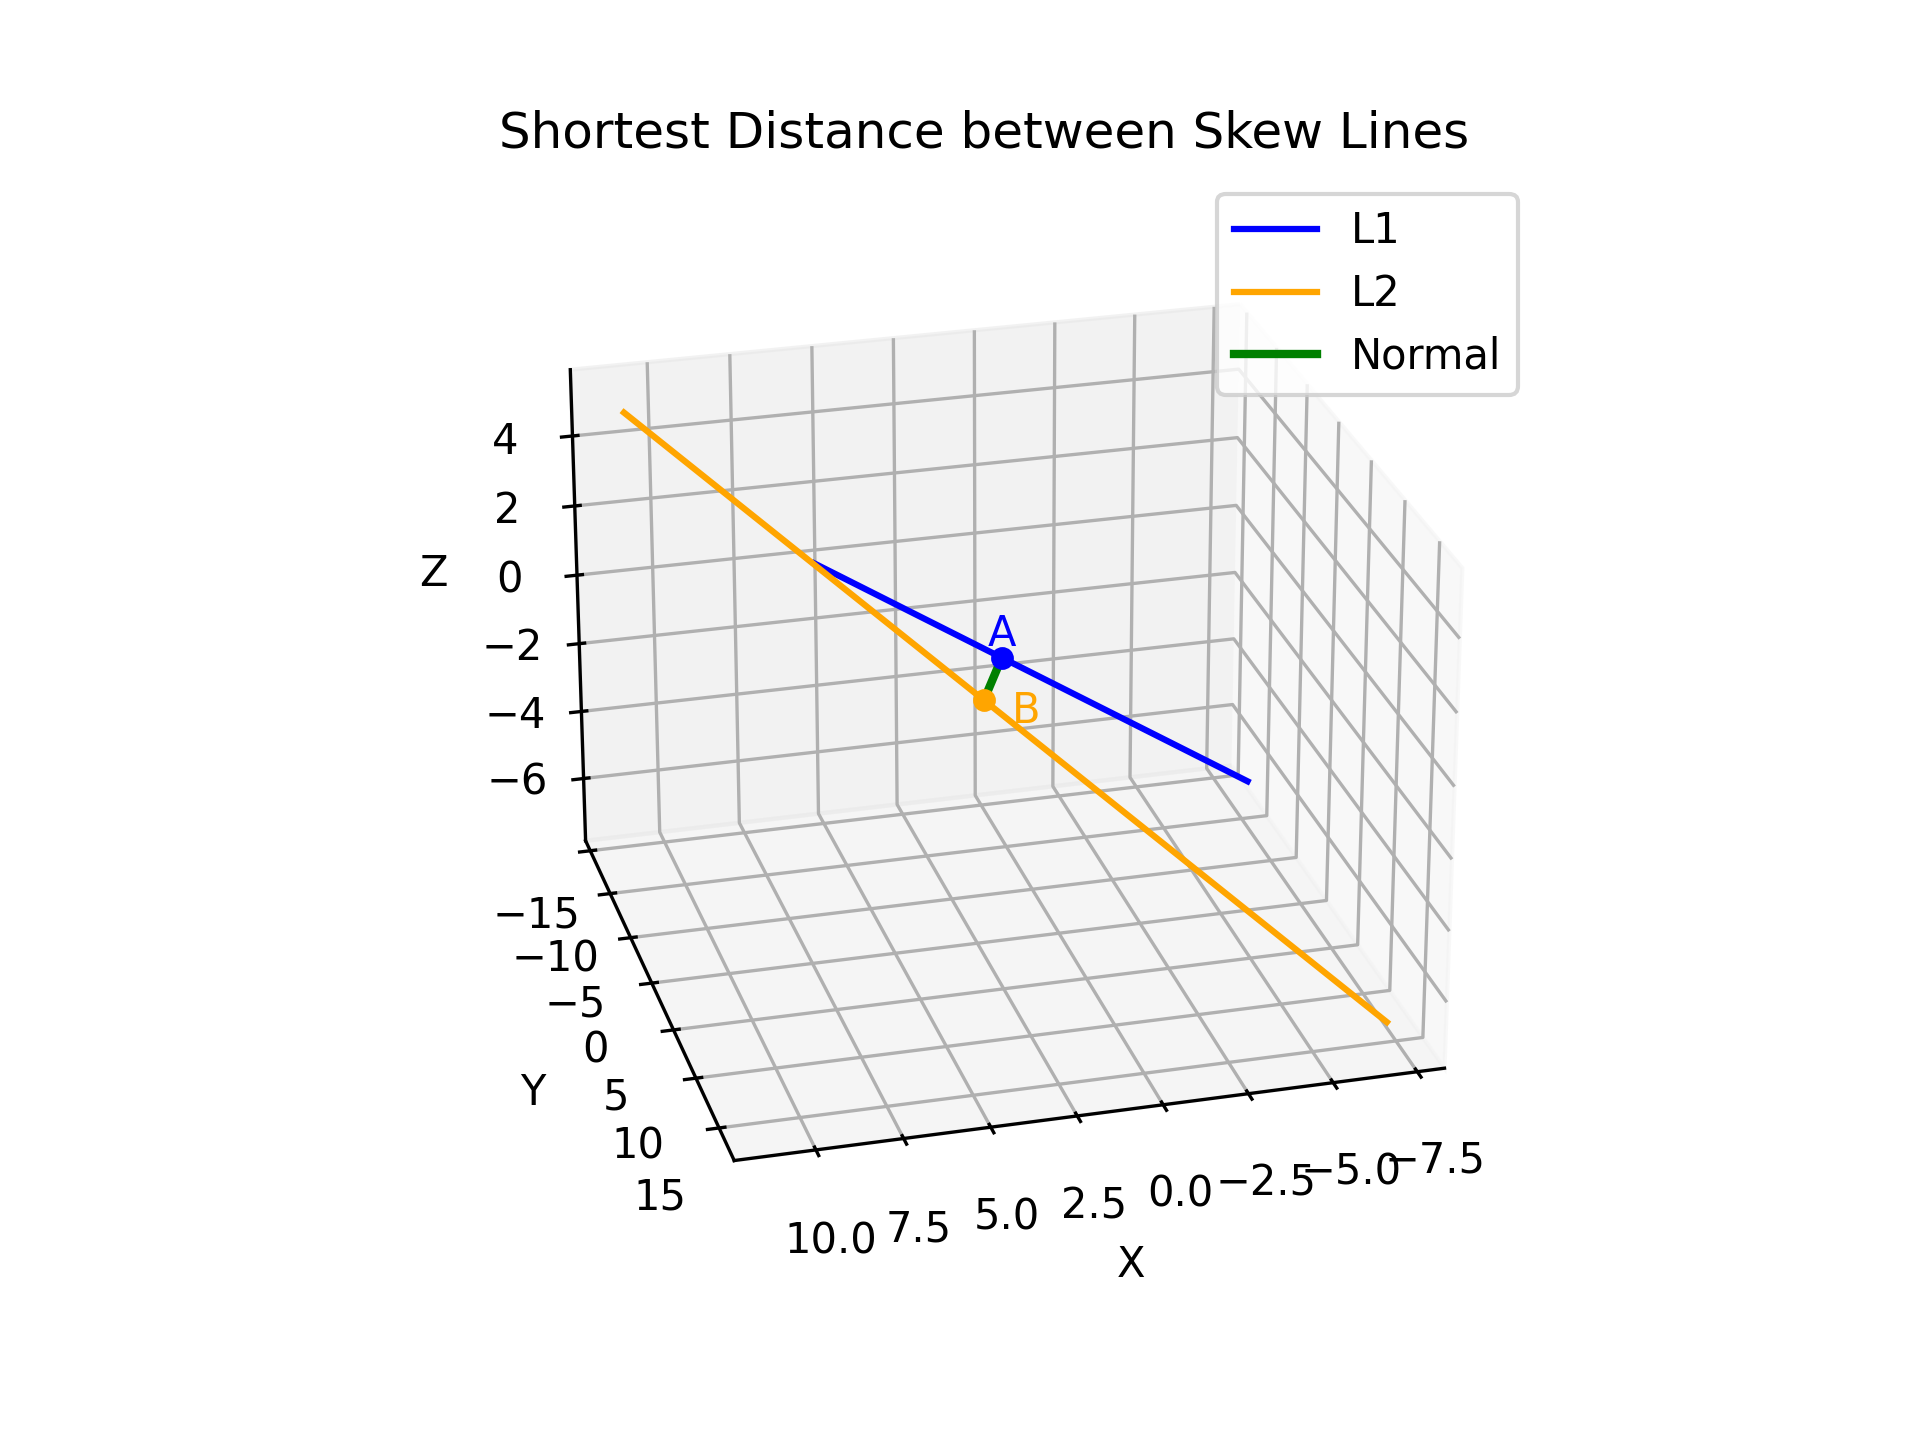
\includegraphics[width=1.2\linewidth]{figs/fig.png}
    \caption{}
    \label{fig:3DVectors}
\end{figure}

\end{document}

